\chapter{Union-Find}
\label{ch:unionfind}

\newcommand{\lecnum}{26}
%\newcommand{\lectitle}{Union-Find}
\newcommand{\lecturer}{Frank Pfenning, Iliano Cervesato}

\chapterTAGS{application, complexity, graph-representation, spanning-tree, union-find}
\maketitle

\begin{preamble}
\noindent
Kruskal's algorithm for minimum weight spanning trees starts with a
collection of single-node trees and adds edges until it has
constructed a spanning tree.  At each step, it must decide if adding
the edge under consideration would create a cycle.  If so, the edge
shall not be added to the spanning tree; if not, it will.

In this lecture we will consider an efficient data structure for
checking if adding an edge to a partial spanning tree would create a
cycle, a so-called \emph{union-find} structure.
\end{preamble}

\begin{gram}[Learning Goals]
This lecture fits  our learning goals as follows.
\begin{description}
\item[Computational Thinking: ]%
  We complete our overview of graphs with union-find, a data structure often
  used when working with graphs.
\item[Algorithms and Data Structures: ]%
  Union-find is an important data structure beyond graphs as it allows to work
  efficiently with equivalence classes whenever we can easily designate an
  element as a canonical representative of the class.
\item[Programming: ]%
  We leave it to the reader to study the code that implements union-find.
\end{description}
\end{gram}


\section{Maintaining Equivalence Classes}
\label{sec:unionfind:equiv_classes}
\TAGS{application, spanning-tree, union-find}

The basic idea behind the union-find data structure is to maintain
equivalence classes of nodes, efficiently.  An equivalence class is a
set of elements related by an \emph{equivalence relation}, which must
be \emph{reflexive}, \emph{symmetric}, and \emph{transitive}.  In our
case, this equivalence relation is defined on nodes in a partial
spanning tree, where two nodes are related if there is a path between
them.  This is reflexive, because from each node $u$ we can reach $u$
by a path of length 0.  It is symmetric because we are working with
undirected graphs, so if $u$ is connected to $w$, then $w$ is also
connected to $u$.  It is transitive because if there is a path from
$u$ to $v$ and one from $v$ to $w$, then the concatenation is a path
from $u$ to $w$.

Initially in Kruskal's algorithm, each node is in its own equivalence
class.  When we connect two trees with an edge, we have to form the
\emph{union} of the two equivalence classes, because each node in
either of the two trees is now connected to all nodes in both trees.

When we have to decide if adding an edge between two nodes $u$ and $w$
would create a cycle, we have to \emph{find} out if $u$ and $w$ belong
to the same equivalence class.  If so, then there is already a path
between $u$ and $w$; adding the edge would create a cycle.  If not,
then there is not already such a path, and adding the edge would
therefore not create a cycle.

The union-find data structure maintains a so-called \emph{canonical
  representative} for each equivalence class, which can be computed
efficiently from any element in the class.  We then determine if two
nodes $u$ and $w$ are in the same class by computing the canonical
representatives of $u$ and $w$, respectively, and comparing them.
If they are equal, they must be in the same class, otherwise they
are in two different classes.


\section{An Example}
\label{sec:unionfind:example}
\TAGS{application, complexity, graph-representation, union-find}

In order to motivate how the union-find data structure works,
we consider an example of Kruskal's algorithm.  We have the following
graph, with the indicated edge weights.
\begin{center}
  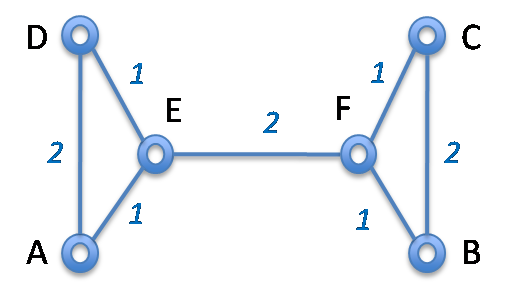
\includegraphics[width=0.45\textwidth]{img/graph1.png}
\end{center}
We have to consider the edges in increasing order, so let's fix the
order $AE$, $ED$, $FB$, $CF$, $AD$, $EF$, $CB$.  We represent the
nodes $A$--$F$ as integers $0$--$5$.

How shall we keep track of equivalence classes?  In its simplest form,
the \emph{union-find structure} is just an array with as many
positions as there are vertices in the graph (or elements in the set),
so that each index represents a vertex.  The contents of the array at
position $i$ is the index of the canonical representative of vertex
$i$ (or of another vertex in the same connected component --- see
below).  In particular, if $i$ is a canonical representative, position
$i$ will contain $i$ itself.

Initially, each node is in its own equivalence class.
\begin{center}
  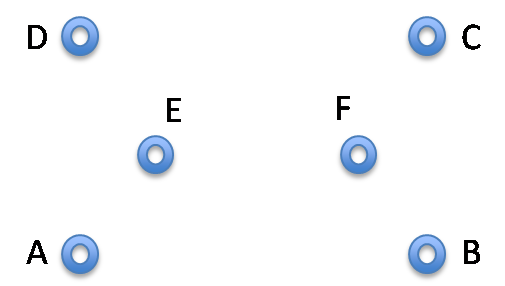
\includegraphics[width=0.45\textwidth]{img/forest0.png}
\end{center}
In the union-find array, $\mathit{UF}$, is in the following state
\begin{center}
  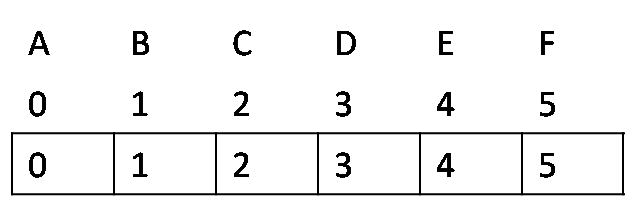
\includegraphics[width=0.6\textwidth]{img/ufs0.png}
\end{center}

We begin by considering the edge $AE$.  We see that vertices $A$
(index 0) and $E$ (index 4) are in two
different equivalence classes because $\mathit{UF}[0] = 0$ and $\mathit{UF}[4] = 4$,
and $0 \neq 4$.  This means we have to add an edge between
$A$ and $E$.
\begin{center}
  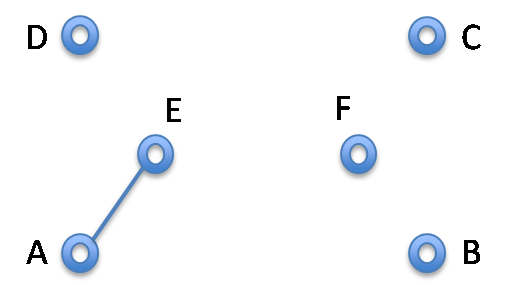
\includegraphics[width=0.45\textwidth]{img/forest1.png}
\end{center}
In the array of canonical representatives, we either have to set
$\mathit{UF}[0] = 4$ or $\mathit{UF}[4] = 0$, depending on whether we choose 4 or 0 as
the representative the new class containing $A$ and $E$.  Let's assume
it's 0.  The array then would be the following:
\begin{center}
  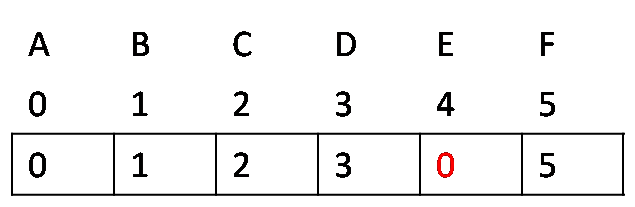
\includegraphics[width=0.6\textwidth]{img/ufs1.png}
\end{center}
where we highlighted the change in \textcolor{red}{red}.  It is
convenient to visualize the contents of the union-find structure as a
\emph{directed} graph with the same vertices as our original graph,
and an edge from $i$ to $j$ exactly when $\mathit{UF}[i]$ contains $j$.  We
display this new graph in \textcolor{green}{green} to distinguish it
from both the original graph and the spanning tree we are
constructing.
\begin{center}
  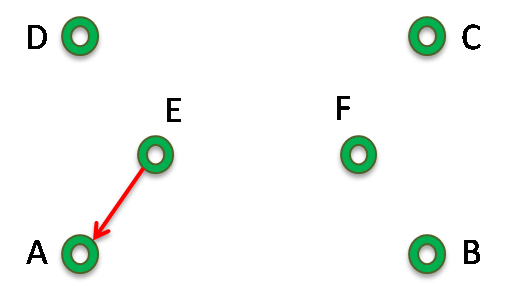
\includegraphics[width=0.35\textwidth]{img/ufg1.png}
\end{center}
The sole purpose of this graph is to make it easier for us humans to
visualize the contents of the union-find structure as we simulate the
union-find algorithm.  An implementation would operate exclusively on
the array.  From now on, we will display the two representations side
by side.  They carry the same information --- you can follow the
discussion on the one that works best for you.


Next we consider $ED$.  Again, this edge should be added because
$\mathit{UF}[4] = 0 \neq 3 = \mathit{UF}[3]$.
\begin{center}
  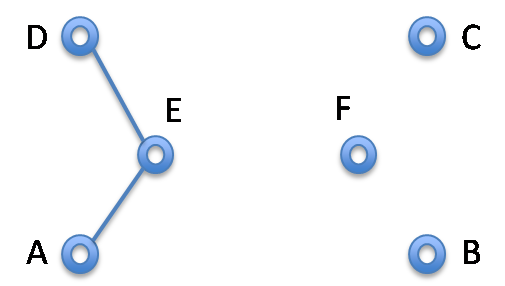
\includegraphics[width=0.45\textwidth]{img/forest2.png}
\end{center}
The union-find structure tells us that $A$ is the canonical
representative of the tree with vertices $A$ and $E$, and $D$ is the
canonical representative of the singleton tree containing just $D$.
Which vertex should we appoint as the canonical representative of the
combined tree?  $E$ is not a good candidate because that would involve
making two changes in the array (both $\mathit{UF}[0]$ and $\mathit{UF}[3]$ would need
to be set to 4).  In general, we want to appoint one of the existing
canonical representatives as the canonical representative of the
combined equivalence class: in this way a single array cell needs to
be modified.  As we are learning our way around union-find, we will
pick $D$ to be the new representative, although we will see later that
this may not be the best choice.  Therefore, we change $\mathit{UF}[0]$ to 3.
The union-find structure now looks as follows:
\begin{center}
  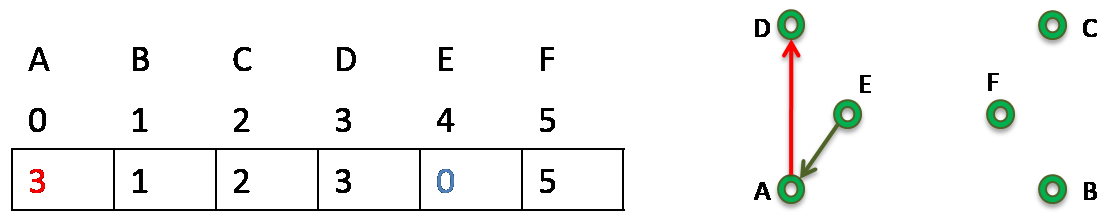
\includegraphics[width=0.99\textwidth]{img/ufsg2.png}
\end{center}
Notice that now $\mathit{UF}[4]$ does not contain any more the canonical
representative of $E$: it points to a vertex from where we can find
its canonical representative.  In general, going through the array and
repointing all vertices to their canonical representative would be
very expensive, although we partially revisit this idea later on.
Observe also that the edge added to the (directed) union-find
visualization graph is different from the edge inserted in the
spanning tree: these two graphs do not carry the same information.

We now combine two more steps, because they are analogous to the above,
adding edges $FB$ and $CF$.
\begin{center}
  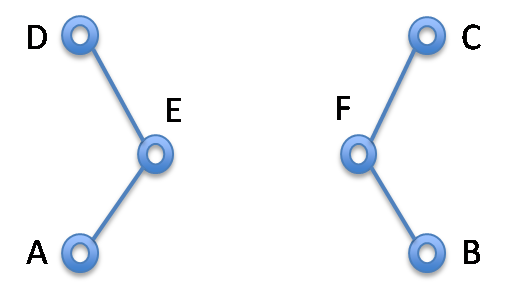
\includegraphics[width=0.45\textwidth]{img/forest4.png}
\end{center}
Again we have some choices.  Let's say the union-find structure
becomes:
\begin{center}
  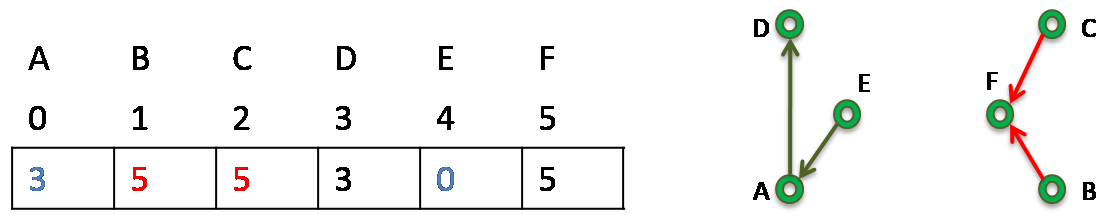
\includegraphics[width=0.99\textwidth]{img/ufsg4.png}
\end{center}

Next was the edge $AD$.  In the array we have that $\mathit{UF}[0] = 3 =
\mathit{UF}[3]$, so $A$ and $D$ belong to the same equivalence class.  Adding
the edge would create a cycle, so we ignore it and move on.

The next edge to consider is $EF$.  Since $\mathit{UF}[4] = 0$ and $\mathit{UF}[0] = 3
\neq 5 = \mathit{UF}[5]$ they are in different equivalence classes.  We shall
appoint one among $D$ and $F$ as the canonical representative of the
combined class.  We arbitrarily choose $F$.  Taking this step we now
have the tree
\begin{center}
  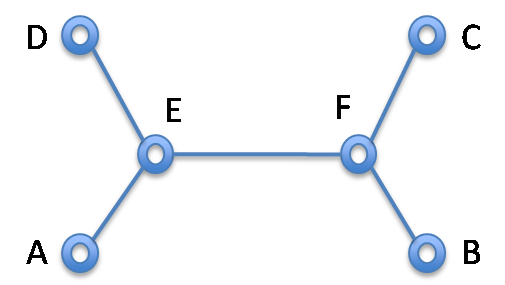
\includegraphics[width=0.45\textwidth]{img/forest5.png}
\end{center}
and a union-find structure which is as follows:
\begin{center}
  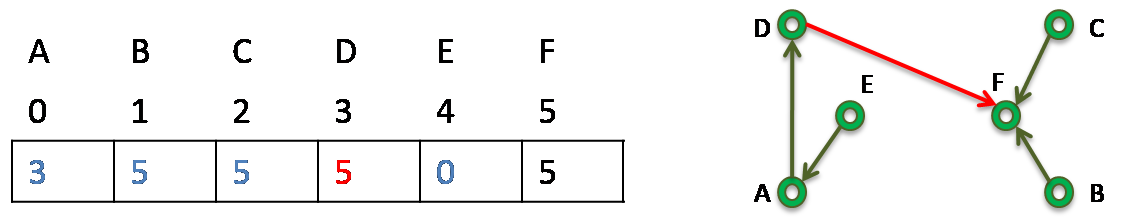
\includegraphics[width=0.99\textwidth]{img/ufsg5.png}
\end{center}
Observe that the edge added to the visualization graph is not in the
original graph.

At this point we can stop, and we don't even need to consider the last
edge $BC$.  That's because we have already added $5 = v-1$ edges
(where $v$ is the number of nodes), so we must have a spanning tree at
this stage.

\medskip%
How does union-find affect the cost of determining whether two
vertices are connected in a graph?  We first need to find their
canonical representatives.  Doing so has a maximum cost of $O(v)$ for
each of them, since we may need to chase (nearly) every vertex in the
graph to reach its canonical representative.  Therefore, checking
whether these vertices are connected costs $O(v)$, which is what we
were able to achieve using BFS (recall that we checked connectivity on
the spanning tree under construction, not on the original graph).
If they are not connected, updating the union-find structure through a
union operation has cost $O(1)$ --- we are just modifying one value in
the array.

Thus, adopting union-find as part of Kruskal's algorithm does not
change the complexity, which remains $O(e \log e + ev)$ or,
simplifying, $O(ev)$.


\section{Height Tracking}
\label{sec:unionfind:height_tracking}
\TAGS{complexity, union-find}

Can we do better?

The cost of the find operation is given by how many vertices we need
to examine to get to the canonical representative of a node.  The
fewer number of intermediate vertices the faster this will be.

It is useful to look at the graphical representation of the union-find
structure as a set of trees, each with its canonical representative as
its root.  Then, the find operation amounts to following edges to the
root of a tree.  Its cost is therefore given by the height of the
tree, i.e., the longest path from a leaf to the root.

The union operation merges one tree into another.  Key to an efficient
find operation is therefore to keep the height of the merged tree as
small as possible.  This insight determines an improved strategy for
merging two trees, $T_1$ of height $h_1$ and $T_2$ of height $h_2$:
\begin{itemize}
\item%
  If $h_1 > h_2$, merge $T_2$ into $T_1$ by appointing the root of
  $T_1$ as the canonical representative of the combined tree.  The
  resulting tree will have height $h_1$.
\item%
  If $h_1 < h_2$, proceed the opposite way and pick the root of $T_2$
  as the root of the merged tree, which will have height $h_2$.
\item%
  If $h_1 = h_2$, it doesn't matter which tree we merge into which:
  the combined tree will have height $h_1 + 1$.
\end{itemize}
Let's apply this strategy on our ongoing example.  When adding edge
$ED$ on the second step, we would appoint $A$ rather than $D$ as the
representative of the new tree, which would give it height 1 instead
of 2.  These were the kind of choices we made when adding edges $FB$
and $CF$.  On the final step, when adding edge $EF$, we would have to
merge two trees of height 1, and so it doesn't matter which way we go:
the resulting tree will have height 2.  Merging the tree rooted at $F$
into the tree rooted at $A$, the final union-find structure is as
follows:
\begin{center}
  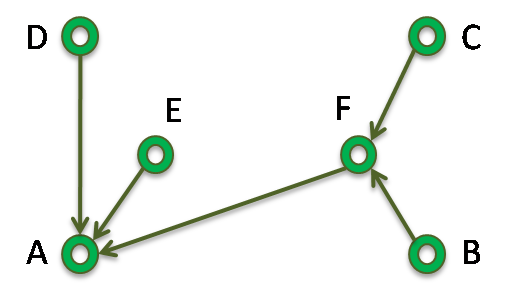
\includegraphics[width=0.35\textwidth]{img/ufg5-ht.png}
\end{center}

To implement this strategy, we need to record the height of each tree
in the union-find structure.  We can still store a single number in
each position of the array by observing that we need to know the
height of a tree only when reaching its root (so that we can decide
which way to merge two trees) and that recording the fact that $i$ is
the root of a tree by storing $i$ in $\mathit{UF}[i]$ is overkill: a simple
flag is enough.  Whenever $i$ is the root of a tree, this suggests
setting $\mathit{UF}[i] = -h$ where $h$ is the height of this tree --- we use
the sign bit as our flag.  Positions that do not correspond to roots
store indices of their parent in the tree, as we did in our first
version of union-find.

Applying this idea to our ongoing example, the $\mathit{UF}$ array evolves as
follows:
\begin{center}
  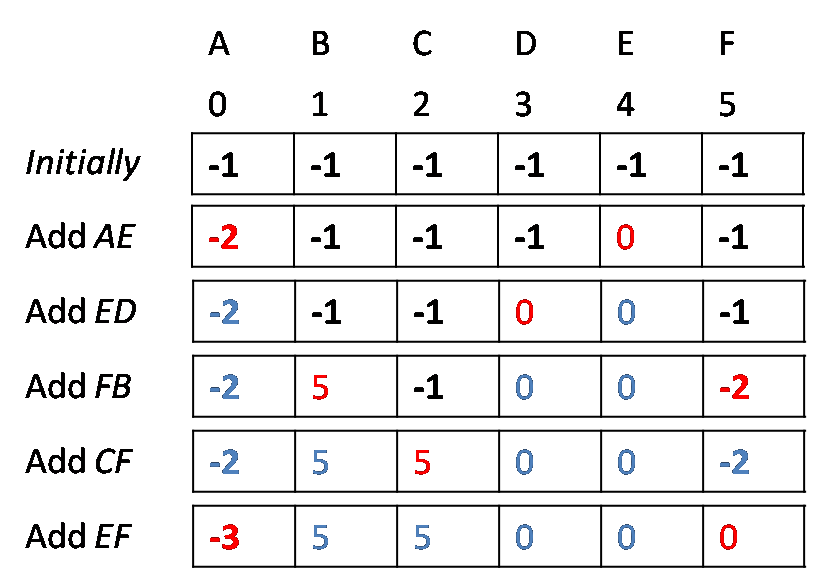
\includegraphics[width=0.75\textwidth]{img/ufs-ht.png}
\end{center}
Here, we highlight in red the changed at each step and use bold to
further emphasize canonical representatives.

Does using this strategy, known as \emph{height tracking}, lower the
cost of the find operation?  To figure this out, we need to understand
what the maximum height of a tree with $v$ nodes can be.  The
following property gives us a way to answer this question:
\begin{quote}\em
  A tree of height $h$ has at least $2^{h-1}$ nodes.
\end{quote}
The proof proceeds by a simple induction on $h$:
\begin{description}
\item[Base case: $h=1$] %
  A tree of height 1 has exactly one node.  And indeed $2^{1-1} = 2^0
  = 1$.

\item[Inductive case: $h > 1$] %
  We need to distinguish subcases on how this tree came about.  This
  tree was constructed by merging two trees, $T_1$ of height $h_1$
  and $T_2$ of height $h_2$.
  \begin{itemize}
  \item%
    If $h_1 > h_2$, then $h = h_1$.  We know that $T_1$ contained at
    least $2^{h-1}$ nodes and therefore the combined tree contains all
    these $2^{h-1}$ nodes plus the nodes of $T_2$.
  \item%
    If $h_1 < h_2$, the argument is symmetric.
  \item%
    If $h_1 = h_2$, then $h = h_1 + 1$.  Thus the merged tree contains
    at least $2^{h-2} + 2^{h-2} = 2^{h-1}$ nodes.
  \end{itemize}
\end{description}

If a tree of height $h$ contains \emph{at least} $2^{h-1}$ vertices,
then a tree with $v$ nodes has height \emph{at most} $\log v$.
Consequently, the find operation of union-find has cost $O(\log v)$.
Thus, using union-find with height tracking lowers the cost of
computing a minimum spanning tree using Kruskal's algorithm to $O(e
\log e + e \log v)$.  Now, since $e$ is at most $v(v-1)/2$, we have
that $e \in O(v^2)$, and therefore $e \log e \in O(e \log v)$ since
$\log v^2 = 2\log v$.  Thus, the overall cost of our algorithm reduces
to $O(e \log v)$, which is an upper bound on the cost of sorting the
edges of the original graph.


\section{Path Compression}
\label{sec:unionfind:path_compression}
\TAGS{complexity, union-find}

Can we do even better?

A further optimization comes from the observation that when finding
the canonical representative of a node, we have the opportunity to
update every node in the path to point directly to the root of the
tree:
\begin{center}
  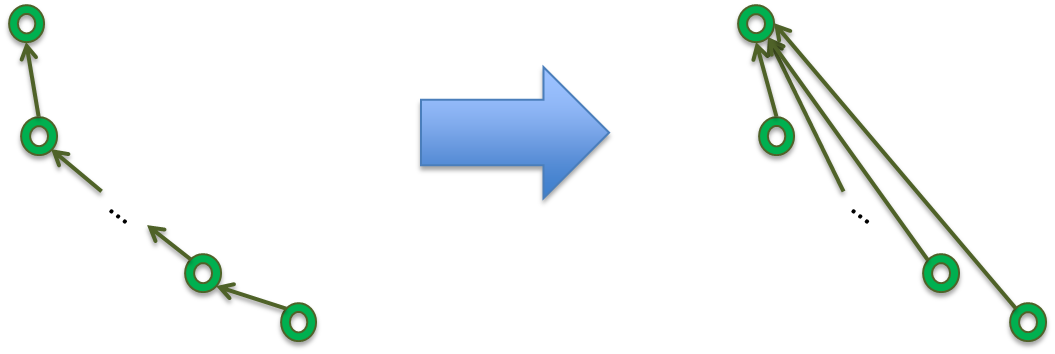
\includegraphics[width=0.9\textwidth]{img/ufg-pc.png}
\end{center}
In this way, any future find operation that involves one of these
nodes will be one hop away from the root.  This will also often
reduce the height of the tree, sometimes dramatically.

This optimization, known as \emph{path compression}, gives the find
operation a nearly-constant amortized complexity.  For a graph with
$v$ vertices, the amortized cost of union-find with height tracking
and path compression is in $O(1 + A^{-1}(v))$, the inverse of the
function $A(v)$ which is equal to $A(n) = \mathit{Ack}(n,n)$.  The function
$\mathit{Ack}(m,n)$ is known as the \emph{Ackermann function}, defined as
follows:
$$
\mathit{Ack}(m,n) =
\left\{
\begin{array}{ll}
   n+1 & \text{if } m=0
\\ \mathit{Ack}(m-1, 1) & \text{if } m > 0 \text{ and } n = 0
\\ \mathit{Ack}(m-1, \mathit{Ack}(m,n-1)) & \text{if } m > 0 \text{ and } n > 0
\end{array}
\right.
$$
This function grows very fast: $\mathit{Ack}(0,0) = 1$, $\mathit{Ack}(1,1) = 3$, $\mathit{Ack}(2,2) =
7$, $\mathit{Ack}(3,3) = 61$, $\mathit{Ack}(4,4)$ is larger than the number of
atoms in the universe.  Therefore, $1 + \mathit{Ack}^{-1}(n,n)$ is nearly 1 for all
practical purposes.


\section{An Implementation}
\label{sec:unionfind:implementation}
\TAGS{union-find}

Instead of developing the implementation here, we refer the reader to the code
on the course web site.

A first implementation, \lstinline'unionfind-lin.c', does not track
the height of the trees, and is therefore linear in the worst case.
It does perform a weak form of path compression: a postcondition of
\lstinline'ufs_find(eqs, i)' is that %
\lstinline'eqs->A[i] == ufs_find(eqs, i)'. That is, before returning
the representative for \lstinline'i', the implementation stores that
representative at \lstinline'A[i]'. This shortens the search time for
subsequent find operations on \lstinline'i'. (See the exercises for
strong path compression.)

A second implementation, \lstinline'unionfind-log.c', changes the
representation to use height tracking as discussed above.  This allows
us to make a quick decision how to pick a representative for the
union.

\clearpage
\section{Exercises}
\label{sec:unionfind:exercises}

\begin{exercise}
  \label{exc:ufs-log}
  Prove that after $n$ union operations, the longest chain from an element to
  its representative is $O(\log n)$ if we always take care to have the class
  with longer chains be the canonical representative of the union.  This is
  without any form of path compression.  Since $n$ is bounded by the
  number $v$ of vertices of the graph, the length of this chain is $O(v)$.
\end{exercise}

\begin{exercise}
  Modify the simple implementation in \lstinline'unionfind-lin.c'
  so it does strong path compression, which means that on every find
  operation, every intermediate node will be redirected to point
  directly to its canonical representative.
\end{exercise}

\begin{exercise}
  Modify the more efficient implementation at \lstinline'unionfind-log.c' to
  do path compression.  Note that this may require loosening the invariants,
  since in the straightforward implementation the stored number is only a
  bound on the longest path and may not be exact (since the path may be
  compressed).
\end{exercise}

% \clearpage
% \bibliographystyle{alpha}
% \bibliography{modal}

% \cleardoublepage
